\documentclass{kthreport}

\usepackage[parfill]{parskip}
\usepackage{subcaption}


\title{Classification of ImageNet with Convolutional Neural Networks}
\subtitle{A study in techniques to improve CNN's}
\author{W. Skagerström, T. Price, N. Lindqvist}
\diarienr{Deepl-18 Project}

\begin{document}
\maketitle


This report is our final piece of work in the course DD2424, Deep Learning in Data Science. The overarching purpose is investigating convolutional neural networks (CNN's) while applying knowledge and techniques which we've acquired in during the course.

To thoroughly investigate the topic a CNN will be constructed in the most vanilla way possible. Different architectures is compared to another before moving on with one which performs better in terms of accuracy. In turns the network will be optimized by more sophisticated initialization, changing activation functions and dropout layers. Each modification and effect will be analyzed. Lastly, the results is discussed on their own and in context of other imageNet classifiers.


\section{Implementing a CNN}

\subsection{Evaluation architectures}

The basis of the CNN architecture is inspired by \cite{NIPS2012_4824}, it is summarized in figure \ref{fig:architecture}. However, it was implemented on the full dataset which features images of resolution $224\times224\times3$ while our images are $64\times64\times3$. Inspired by \textbf{insert 3 reports here} we decided to test three configurations, summarized in \ref{table:configurations}.

\begin{figure}[htbp]
  \centering
  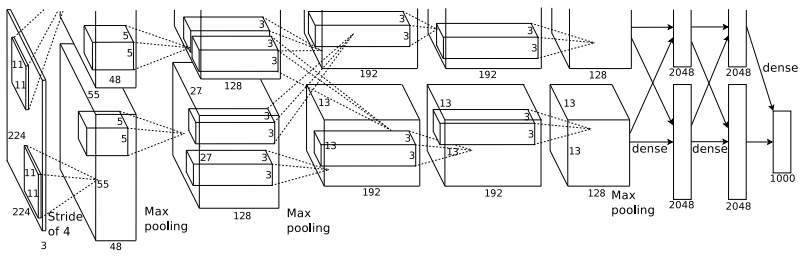
\includegraphics[width=\linewidth]{../images/architecture.jpg}
  \caption[]
  {\small
    Overview of network architecture presented by \cite{NIPS2012_4824}.
  }
  \label{fig:architecture}
\end{figure}


Tests was run with \textbf{insert how tests were run, how data was split, validation size, etc.} The results of each architecture is preented in

\subsection{Initialization matters}

Moving on with current architecture of the network we 

\subsection{Implementation specifics}

The stack for implementation consisted of Python, Keras, etc. The test was run on \textbf{[insert hardware]}.


\subsection{First important subtopic}

Lorem Ipsum is simply dummy text of the printing and typesetting industry. Lorem Ipsum has been the industry's standard dummy text ever since the 1500s, when an unknown printer took a galley of type and scrambled it to make a type specimen book. It has survived not only five centuries, but also the leap into electronic typesetting, remaining essentially unchanged. It was popularised in the 1960s with the release of Letraset sheets containing Lorem Ipsum passages, and more recently with desktop publishing software like Aldus PageMaker including versions of Lorem Ipsum.



\section{Discussion}

\subsection{Evaluation out results}

Lorem ipsum dolor sit amet.

\subsection{ImageNet state of the art}

Lorem ipsum dolor sit amet.



\bibliography{references}{}
\bibliographystyle{plain}

\end{document}
